\documentclass[10pt,a4paper]{article}
\usepackage[utf8]{inputenc}
\usepackage{graphicx}
\def\Pr{\mathop{\rm Pr}}
\usepackage[landscape,margin=1cm]{geometry}
\usepackage[english]{babel}
\usepackage{tikz,listings}
\usepackage{musicography}
\usepackage{listofitems} % for \readlist to create arrays
\usetikzlibrary{arrows,snakes,backgrounds,shapes.geometric}
\tikzstyle{mynodegreen}=[thick,draw=green,fill=blue!20,circle,minimum size=22]
\tikzstyle{mynode}=[thick,draw=blue,fill=blue!20,circle,minimum size=22]
\tikzstyle{mynodered}=[thick,draw=red,fill=blue!20,circle,minimum size=22]
\usepackage{xcolor}
\colorlet{myred}{red!80!black}
\colorlet{myblue}{blue!80!black}
\colorlet{mygreen}{green!60!black}
\colorlet{myorange}{orange!70!red!60!black}
\colorlet{mydarkred}{red!30!black}
\colorlet{mydarkblue}{blue!40!black}
\colorlet{mydarkgreen}{green!30!black}
\tikzstyle{node}=[thick,circle,draw=myblue,minimum size=22,inner sep=0.5,outer sep=0.6]
\tikzstyle{node in}=[node,green!20!black,draw=mygreen!30!black,fill=mygreen!25]
\tikzstyle{node hidden}=[node,blue!20!black,draw=myblue!30!black,fill=myblue!20]
\tikzstyle{node convol}=[node,orange!20!black,draw=myorange!30!black,fill=myorange!20]
\tikzstyle{node out}=[node,red!20!black,draw=myred!30!black,fill=myred!20]
\tikzstyle{connect}=[thick,mydarkblue] %,line cap=round
\tikzstyle{connect arrow}=[-{Latex[length=4,width=3.5]},thick,mydarkblue,shorten <=0.5,shorten >=1]
\tikzset{ % node styles, numbered for easy mapping with \nstyle
  node 1/.style={node in},
  node 2/.style={node hidden},
  node 3/.style={node out},
}
\def\nstyle{int(\lay<\Nnodlen?min(2,\lay):3)} % map layer number onto 1, 2, or 3

\input{neuromatch-template.tex}
\clearpage
\begin{document}
%\let\clearpage\relax
\includegraphics[scale=0.03]{Figures/NMADL.png}\href{https://compneuro.neuromatch.io/tutorials/intro.html}{\textbf{\Huge{Neuromatch Academy: Basics and Pytorch - Summary Sheet}}}
\small
\begin{multicols}{3}
\begin{textbox}{\href{https://deeplearning.neuromatch.io/tutorials/W1D1_BasicsAndPytorch/student/W1D1_Tutorial1.html}{Pytorch (W1D1T1) }}
\begin{subbox}{subbox}{Neuromatch Academy Contributors}
\scriptsize
\textbf{Content creators:} Shubh Pachchigar, Vladimir Haltakov, Matthew Sargent, Konrad Kording\\
\textbf{Content reviewers:} Deepak Raya, Siwei Bai, Kelson Shilling-Scrivo\\
\textbf{Content editors:} Anoop Kulkarni, Spiros Chavlis\\
\textbf{Production editors:} Arush Tagade, Spiros Chavlis

\end{subbox}
\begin{subbox}{subbox}{The Basics of PyTorch}
\scriptsize


PyTorch is a Python-based scientific computing package targeted at two sets of audiences:
\begin{itemize}
    \item 
A replacement for NumPy optimized for GPUs
    \item A deep learning platform that provides significant flexibility and speed
\end{itemize}
At its core, PyTorch provides a few key features:

\begin{itemize}
    \item A multidimensional Tensor object, similar to NumPy Array but with GPU acceleration.
    \item An optimized autograd engine for automatically computing derivatives.
    \item A clean, modular API for building and deploying deep learning models.
\end{itemize}



\end{subbox}
%%%%% Creating Tensors
\begin{subbox}{subbox}{Creating Tensors}
\scriptsize
Tensors, which are like vector are the building blocks of pyTorch.
There are various ways of creating tensors, and when doing any real deep learning project, we will usually have to do so. Construct tensors directly:

\begin{lstlisting}[language=Python]
# We can construct a tensor directly from 
# some common python iterables,
# such as list and tuple nested iterables 
# can also be handled as long as the
# dimensions are compatible
# tensor from a list
a = torch.tensor([0, 1, 2])
#tensor from a tuple of tuples
b = ((1.0, 1.1), (1.2, 1.3))
b = torch.tensor(b)
# tensor from a numpy array
c = np.ones([2, 3])
c = torch.tensor(c)
\end{lstlisting}
Creating random tensors and tensors like other tensors:
\begin{lstlisting}[language=Python]
# There are also constructors for random numbers
# Uniform distribution
a = torch.rand(1, 3)
# Normal distribution
b = torch.randn(3, 4)
\end{lstlisting}
\end{subbox}
\end{textbox}
%%%%%%%%%%%%%%%%%%%%%%%%%%%%%%%%%%%%%%%%%%%%%%%%%%
\begin{textbox}{\href{https://deeplearning.neuromatch.io/tutorials/W1D1_BasicsAndPytorch/student/W1D1_Tutorial1.html}{Pytorch (W1D1T1) }}
\begin{subbox}{subbox}{Tensor Operations in PyTorch}
\scriptsize
We can perform operations on tensors using methods under `torch.`

\begin{lstlisting}[language=Python]
# addition of a and b this only works if c already exist
torch.add(a, b, out=c)

# Pointwise Multiplication of a and b
torch.multiply(a, b, out=d)

\end{lstlisting}
In PyTorch, most common Python operators are overridden.
The common standard arithmetic operators ($+$, $-$, $*$, $/$, and $**$) have all been lifted to elementwise operations.
\begin{lstlisting}[language=Python]
x = torch.tensor([1, 2, 4, 8])
y = torch.tensor([1, 2, 3, 4])
x + y=tensor([ 2,  4,  7, 12]),
x - y= tensor([0, 0, 1, 4]),
x * y= tensor([ 1,  4, 12, 32]),
x / y= tensor([1.0000, 1.0000, 1.3333, 2.0000]),
x**y = tensor([   1,    4,   64, 4096]))
\end{lstlisting}
\textbf{Tensor Methods}

Tensors also have a number of common arithmetic operations built in, like x.sum() or x.mean(). A list of methods can be found  in the appendix (there are a lot!).

\textbf{Matrix Operations}

The \textit{$@$} symbol is overridden to represent matrix multiplication. You can also use `torch.matmul()` to multiply tensors. For dot multiplication, you can use `torch.dot()`, or manipulate the axes of your tensors and do matrix multiplication. 

Transposes of 2D tensors are obtained using `torch.t()` or `Tensor.T`. Note the lack of brackets for `Tensor.T` - it is an attribute, not a method.

\end{subbox}
\end{textbox}
%%%% MANIPULATION
\begin{textbox}{\href{https://deeplearning.neuromatch.io/tutorials/W1D1_BasicsAndPytorch/student/W1D1_Tutorial1.html}{Pytorch (W1D1T1) }}

\begin{subbox}{subbox}{Manipulating Tensors in Pytorch}
\scriptsize
\textbf{Indexing}

Just as in numpy, elements in a tensor can be accessed by index. As in any numpy array, the first element has index 0 and ranges are specified to include the first to last\_element-1. We can access elements according to their relative position to the end of the list by using negative indices. Indexing is also referred to as slicing.\\

\textbf{Flatten and reshape}

There are various methods for reshaping tensors. It is common to have to express 2D data in 1D format. Similarly, it is also common to have to reshape a 1D tensor into a 2D tensor. We can achieve this with the `.flatten()` and `.reshape()` methods.\\

\textbf{Squeezing tensors}

When processing batches of data, you will quite often be left with singleton dimensions. E.g., `[1,10]` or `[256, 1, 3]`. This dimension can quite easily mess up your matrix operations if you don't plan on it being there...\\



\textbf{Permutation}

Sometimes our dimensions will be in the wrong order! For example, we may be dealing with RGB images with dim $[3\times48\times64]$, but our pipeline expects the colour dimension to be the last dimension, i.e., $[48\times64\times3]$. To get around this we can use the `.permute()` method.\\

\textbf{Concatenation}

Two matrices can be concatenated along rows (axis 0, the first element of the shape) vs. columns (axis 1, the second element of the shape) using  `torch.cat((x, y), dim=0)`.\\


\textbf{Conversion to Other Python Objects}

Converting a tensor to a numpy.ndarray, or vice versa, is easy, and the converted result does not share memory. This minor inconvenience is quite important: when you perform operations on the CPU or GPUs, you do not want to halt computation, waiting to see whether the NumPy package of Python might want to be doing something else with the same chunk of memory.

When converting to a NumPy array, the information being tracked by the tensor will be lost.

\end{subbox}
\end{textbox}

\end{multicols}
\begin{multicols}{3}
\begin{textbox}{\href{https://deeplearning.neuromatch.io/tutorials/W1D1_BasicsAndPytorch/student/W1D1_Tutorial1.html}{Pytorch (W1D1T1) }}
\begin{subbox}{subbox}{Graphics processing unit (GPU)}
\scriptsize

When using Colab notebooks, by default, will not have access to a GPU. In order to start using GPUs we need to request one. We can do this by going to the runtime tab at the top of the page. 

By following \textbf{Runtime} → \textbf{Change runtime type} and selecting \textit{GPU} from the \textbf{Hardware Accelerator} dropdown list, we can start playing with sending tensors to GPUs.

Once you have done this your runtime will restart and you will need to rerun the first setup cell to re-import PyTorch. Then proceed to the next cell.

For more information on the GPU usage policy you can view in the Appendix.\\

\textbf{Compute Unified Device Architecture (CUDA)}\\

\href{(https://developer.nvidia.com/cuda-toolkit)}{\textbf{CUDA}} is an API developed by Nvidia for interfacing with GPUs. PyTorch provides us with a layer of abstraction, and allows us to launch CUDA kernels using pure Python.

In short, we get the power of parallelizing our tensor computations on GPUs, whilst only writing (relatively) simple Python!

Here, we define the function "set\_device", which returns the device use in the notebook, i.e., "cpu" or "cuda". Unless otherwise specified, we use this function on top of every tutorial, and we store the device variable such as

\begin{lstlisting}[language=Python]
DEVICE = set_device()
\end{lstlisting}

Let's define the function using the PyTorch package `torch.cuda`, which is lazily initialized, so we can always import it, and use `is\_available()` to determine if our system supports CUDA.

\textbf{Operations between CPU tensors and CUDA tensors}

Note that the type of the tensor changed after calling .to(). What happens if we try and perform operations on tensors on devices?

We cannot combine CUDA tensors and CPU tensors in this fashion. If we want to compute an operation that combines tensors on different devices, we need to move them first! We can use the .to() method as before, or the .cpu() and .cuda() methods. Note that using the .cuda() will throw an error, if CUDA is not enabled in your machine.

Generally, in this course, all Deep Learning is done on the GPU, and any computation is done on the CPU, so sometimes we have to pass things back and forth.

\end{subbox}
\end{textbox}

\end{multicols}
\begin{multicols}{3}
\begin{textbox}{Neural Networks}
\begin{subbox}{subbox}{ Introduction}
\scriptsize
Now it’s time for you to create your first neural network using PyTorch. This section will walk you through the process of:
\begin{itemize}
    \item 
Creating a simple neural network model
    \item Training the network
    \item Visualizing the results of the network
    \item Tweaking the network
\end{itemize}
\end{subbox}
\begin{subbox}{subbox}{ Data }
\scriptsize

First we need some sample data to train our network on. The example dataset consists of 2D points along two interleaving half circles, figure below. 

\centering
\includegraphics[scale=0.3]{Figures/NN/NNFigure1.png}

\end{subbox}
%%%%% Create a Simple Neural Network
\begin{subbox}{subbox}{ Create a Simple Neural Network}
\scriptsize
For this example we want to have a simple neural network consisting of 3 layers:

\begin{itemize}
\item
 input layer of size 2 (our points have 2 coordinates)
\item hidden layer of size 16 (you can play with different numbers here)

 \item
 output layer of size 2 (we want the have the scores for the two classes)
 \end{itemize}
 
During the course you will deal with different kinds of neural networks.
\end{subbox}
\end{textbox}
%%%%%%%%%%%%
\begin{textbox}{Create a Simple Neural Network}
\begin{subbox}{subbox}{Programing the Network }
\scriptsize


PyTorch provides a base class for all neural network modules called nn.Module. You need to inherit from nn.Module and implement some important methods:

\begin{itemize}
    \item[
\textbf{init}]
In the \textbf{init} method you need to define the structure of your network. Here you will specify what layers will the network consist of, what activation functions will be used etc.
\item[\textbf{forward}]
All neural network modules need to implement the \textbf{forward} method. It specifies the computations the network needs to do when data is passed through it.
\item[\textbf{predict}]
This is not an obligatory method of a neural network module, but it is a good practice if you want to quickly get the most likely label from the network. It calls the forward method and chooses the label with the highest score.
\item[\textbf{train}]
This is also not an obligatory method, but it is a good practice to have. The method will be used to train the network parameters and will be implemented later in the notebook.
\end{itemize}

\end{subbox}
\begin{subbox}{subbox}{Example Architecture the Network }
\scriptsize
The schematic below shows an example neural network with two nodes in the input layers, four nodes in the hidden layer (in the code there are 16 nodes) and two nodes in the output layer. 
% NEURAL NETWORK no text
\begin{center}
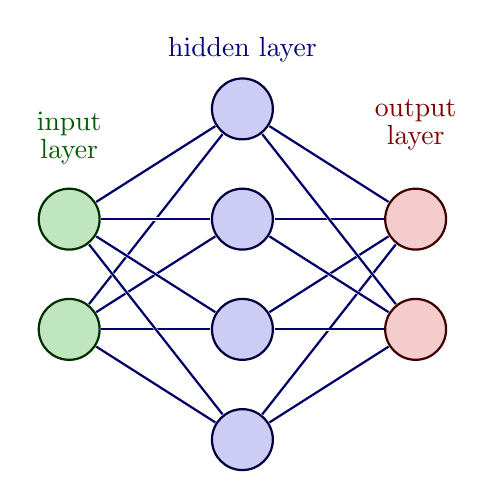
\begin{tikzpicture}[x=2.2cm,y=1.4cm]
  \message{^^JNeural network without text}
  \readlist\Nnod{2,4,2} % array of number of nodes per layer
  
  \message{^^J  Layer}
  \foreachitem \N \in \Nnod{ % loop over layers
    \def\lay{\Ncnt} % alias of index of current layer
    \pgfmathsetmacro\prev{int(\Ncnt-1)} % number of previous layer
    \message{\lay,}
    \foreach \i [evaluate={\y=\N/2-\i; \x=\lay; \n=\nstyle;}] in {1,...,\N}{ % loop over nodes
      
      % NODES
      \node[node \n] (N\lay-\i) at (\x,\y) {};
      
      % CONNECTIONS
      \ifnum\lay>1 % connect to previous layer
        \foreach \j in {1,...,\Nnod[\prev]}{ % loop over nodes in previous layer
          \draw[connect,white,line width=1.2] (N\prev-\j) -- (N\lay-\i);
          \draw[connect] (N\prev-\j) -- (N\lay-\i);
          %\draw[connect] (N\prev-\j.0) -- (N\lay-\i.180); % connect to left
        }
      \fi % else: nothing to connect first layer
      
    }
  }
  
  % LABELS
  \node[above=5,align=center,mygreen!60!black] at (N1-1.90) {input\\[-0.2em]layer};
  \node[above=2,align=center,myblue!60!black] at (N2-1.90) {hidden layer};
  \node[above=10,align=center,myred!60!black] at (N\Nnodlen-1.90) {output\\[-0.2em]layer};
  
\end{tikzpicture}
\end{center}
\end{subbox}
\end{textbox}
\begin{textbox}{Simple Neural Network in python}
\tiny
\begin{lstlisting}[language=Python]
# Inherit from nn.Module - the base class for neural network modules provided by Pytorch
class NaiveNet(nn.Module):
  """
  NaiveNet architecture
  Structure is as follows:
  Linear Layer (2, 16) -> ReLU activation -> Linear Layer (16, 2)
  """
  \end{lstlisting}
\begin{subbox}{subbox}{\textbf{init} function }
\begin{lstlisting}[language=Python]
  # Define the structure of your network
  def __init__(self):
    """
    Defines the NaiveNet structure by initialising following attributes nn.Linear (2, 16):  Transformation from the input to the hidden layer nn.ReLU: Activation function (ReLU) is a non-linearity which is widely used because it reduces computation.
    The function returns 0 if it receives any negative input, but for any positive value x, it returns that value back. 
    nn.Linear (16, 2): Transformation from the hidden to the output layer   
    Args:
      None
    Returns:
      Nothing
    """
    super(NaiveNet, self).__init__()
    # The network is defined as a sequence of operations
    self.layers = nn.Sequential(
        nn.Linear(2, 16),
        nn.ReLU(),
        nn.Linear(16, 2),
    )
\end{lstlisting}
\end{subbox}
\end{textbox}
\begin{textbox}{Simple Neural Network in python}
\tiny
\begin{subbox}{subbox}{\textbf{forward} function }
\begin{lstlisting}[language=Python]
  # Specify the computations performed on the data
  def forward(self, x):
    """
    Defines the forward pass through the above defined structure
    Args:
      x: torch.Tensor
        Input tensor of size ([3])
    Returns:
      layers: nn.module
        Initialised Layers in order to re-use the same layer for each forward pass of data you make.
    """
    # Pass the data through the layers
    return self.layers(x)
\end{lstlisting}
\end{subbox}
\begin{subbox}{subbox}{\textbf{predict} function }
\begin{lstlisting}[language=Python]
  # Choose the most likely label predicted by the network
  def predict(self, x):
    """
    Performs the prediction task of the network
    Args:
      x: torch.Tensor
        Input tensor of size ([3])
    Returns:
      Most likely class i.e., Label with the highest score
    """
    # Pass the data through the networks
    output = self.forward(x)
    # Choose the label with the highest score
    return torch.argmax(output, 1)
\end{lstlisting}
\end{subbox}

\begin{subbox}{subbox}{\textbf{train} function }
\tiny
\begin{lstlisting}[language=Python]
  # Train the neural network (will be implemented later)
  def train(self, X, y):
    """
    Training the Neural Network
    Args:
      X: torch.Tensor (Input data)
      y: torch.Tensor
        Class Labels/Targets
    Returns:
      Nothing
    """
    pass
\end{lstlisting}
\end{subbox}

\end{textbox}
%%%%%%%%%%%%%%%%%%%%%%%%%%%%%%%%%%%%%%%%%%%%%%%%%%
%%%%%%%%%%%%%%%%%%%%%%%%%%%%%%%%%%%%%%%%%%%%%%%%%%
\begin{textbox}{Train Your Neural Network}
\begin{subbox}{subbox}{Train the Network}
\scriptsize
Now it is time to train your network on your dataset. Don’t worry if you don’t fully understand everything yet - we will cover training in much more details in the next days. For now, the goal is just to see your network in action!

You will usually implement the train method directly when implementing your class NaiveNet. Here, we will implement it as a function outside of the class in order to have it in a separate cell. 
\begin{lstlisting}[language=Python]
# Implement the train function given a training dataset X and corresponding labels y
def train(model, X, y):
  """
    Training the Neural Network
    Args:
      X: torch.Tensor
        Input data
      y: torch.Tensor
        Class Labels/Targets
    Returns:
      losses: Float
        Cross Entropy Loss; Cross-entropy builds upon the idea of entropy from information theory and calculates the number of bits required to represent or transmit an average event from one distribution compared to another distribution.
    """
  # The Cross Entropy Loss is suitable for classification problems
  loss_function = nn.CrossEntropyLoss()
  # Create an optimizer (Stochastic Gradient Descent) that will be used to train the network
  learning_rate = 1e-2
  optimizer = torch.optim.SGD(model.parameters(), lr=learning_rate)
  # Number of epochs
  epochs = 15000
  # List of losses for visualization
  losses = []
  for i in range(epochs):
    # Pass the data through the network and compute the loss
    y_logits = model.forward(X)
    loss = loss_function(y_logits, y)
    # Clear the previous gradients and compute the new ones
    optimizer.zero_grad()
    loss.backward()
    # Adapt the weights of the network
    optimizer.step()
    # Store the loss
    losses.append(loss.item())
  return losses
# Create a new network instance a train it
model = NaiveNet().to(DEVICE)
losses = train(model, X, y)
\end{lstlisting}
\end{subbox}
\end{textbox}
%%%%%%%%%%%%%%%%%%%%%%%%%%%%%%%%%%%%%%%%%%%%%%%%%%
%%%%%%%%%%%%%%%%%%%%%%%%%%%%%%%%%%%%%%%%%%%%%%%%%%
%%%%%%%%%%%%%%%%%%%%%%%%%%%%%%%%%%%%%%%%%%%%%%%%%%
%%%%%%%%%%%%%%%%%%%%%%%%%%%%%%%%%%%%%%%%%%%%%%%%%%
\begin{textbox}{Trained Neural Network}
\begin{subbox}{subbox}{The output of the Neural Network}
\scriptsize
The plot below shows the categorisation boundary for the neural network after learning for the two data types (white and black). The neural network does a reasonable job of separating the data.
\begin{center}
\includegraphics[scale=0.28]{Figures/NN/W1D1_Tutorial1_Learnt.png}
\end{center}
The plot below shows the loss during the training to see how it reduces and converges.
\begin{center}
\includegraphics[scale=0.28]{Figures/NN/W1D1_Tutorial1_181_LossFunction.png}
\end{center}

\end{subbox}
\begin{subbox}{subbox}{Tweak your Network}
\scriptsize
You can now play around with the network a little bit to get a feeling of what different parameters are doing. Here are some ideas what you could try:
\begin{itemize}
    \item 
Increase or decrease the number of epochs for training
\item Increase or decrease the size of the hidden layer
\item Add one additional hidden layer
\end{itemize}
Can you get the network to better fit the data?

\end{subbox}
\begin{subbox}{subbox}{W1D1 MusicMatch \musEighth}
\scriptsize
The  
 musical matching for the
 tutorials Basics And Pytorch  is
“Rolling in the Deep” by Adele. 

\end{subbox}
\end{textbox}

%%%%%% APPENDIX
\begin{textbox}{Appendix}
\begin{subbox}{subbox}{ Official PyTorch resources:}
\scriptsize
\begin{itemize}
    \item 
\href{https://pytorch.org/tutorials/}{Pytorch Tutorials}

\item 
\href{https://pytorch.org/docs/stable/tensors.html}{Documentation}

\item  
\href{https://pytorch.org/docs/stable/generated/torch.Tensor.view.html#torch.Tensor.view}{TORCH.TENSOR.VIEW}

\item  
\href{https://pytorch.org/vision/stable/datasets.html}{pre-loaded image datasets}

\end{itemize} 
\end{subbox}
\begin{subbox}{subbox}{ Google Colab Resources:}
\begin{itemize}
    \item 
    \href{https://research.google.com/colaboratory/faq.html}{FAQ including guidance on GPU usage}

 \end{itemize}
\end{subbox}
\begin{subbox}{subbox}{ Books for reference:}
\begin{itemize}
    \item 
    \href{https://www.deeplearningbook.org/}{Deep Learning by Ian Goodfellow, Yoshua Bengio and Aaron Courville}

 \end{itemize}
\end{subbox}
\end{textbox}
\end{multicols}
%\begin{multicols}{3}
\begin{textbox}{Appendix}
\begin{subbox}{subbox}{ Official PyTorch resources:}
\scriptsize
\begin{itemize}
    \item 
\href{https://pytorch.org/tutorials/}{Pytorch Tutorials}

\item 
\href{https://pytorch.org/docs/stable/tensors.html}{Documentation}

\item  
\href{https://pytorch.org/docs/stable/generated/torch.Tensor.view.html#torch.Tensor.view}{TORCH.TENSOR.VIEW}

\item  
\href{https://pytorch.org/vision/stable/datasets.html}{pre-loaded image datasets}

\end{itemize} 
\end{subbox}
\begin{subbox}{subbox}{ Google Colab Resources:}
\begin{itemize}
    \item 
    \href{https://research.google.com/colaboratory/faq.html}{FAQ including guidance on GPU usage}

 \end{itemize}
\end{subbox}
\begin{subbox}{subbox}{ Books for reference:}
\begin{itemize}
    \item 
    \href{https://www.deeplearningbook.org/}{Deep Learning by Ian Goodfellow, Yoshua Bengio and Aaron Courville}

 \end{itemize}
\end{subbox}
\end{textbox}
\end{multicols}
\end{document}
